\documentclass[10pt]{article}
\usepackage{amsmath,amssymb,float, graphicx}
\usepackage[margin=.5in]{geometry}
\pagenumbering{gobble}
\begin{document}

\begin{center}
	\Large Dynamical Research Summer 2014\\
	Singular, Non-Holomorphic Perturbations
\end{center}

\section{Updates/Figures}

\subsection{Weekly Updates}

\textbf{7/6/2014:}

\begin{itemize}
	\item Working through the Bozyck/Peckham paper again for refresher
	\item Worked on the parameter space function and managed to get that to pump out images
	\item Starting using standard ``spectral'' color mapping, added colormap as parameter to functions
	\item Added a kind of general main function through which I can make phase or param space images
	\item Added a filename convention to keep track of what a given image is depicting
	\item Added some code to generate the latex snippet needed to add an image to a latex document
	\item Started a running work pdf to hold weekly updates along with archive-worthy images
	\item Starting to work on solving along the real axis
\end{itemize}

\textbf{8/10/2014:}

\begin{itemize}
	\item Continuing work along the real axis
	\item Solved for fixed point with respect to $c$ and $\beta$
	\item Made orbit diagrams for real case with $c$ varying, may make $\beta$ vary if useful
	\item Tried decomposing singular maps into maps of $\mathbb{R}^2$, not much success
\end{itemize}

\newpage

\subsection{Images}
\vspace{-35pt}
\begin{figure}[H]\centering\includegraphics[width=.6\textwidth]{{param--n=2--d=2--beta=0.000100000000000000--angle=0}.png}\caption{Parameter space image for param $c$ with the equation $z^{2} + 1 + \frac{0.000100000000000000}{ \overline{z}^{2}}$}\end{figure}

\begin{figure}[H]\centering\includegraphics[width=.6\textwidth]{{param--n=2--d=2--beta=0.0100000000000000--angle=0}.png}\caption{Parameter space image for param $c$ with the equation $z^{2} + 1 + \frac{0.0100000000000000}{ \overline{z}^{2}}$}\end{figure}

\begin{figure}[H]\centering\includegraphics[width=.6\textwidth]{{phase--n=2--d=2--beta=-0.00100000000000000--angle=0}.png}\caption{Phase space image of $z^{2} + -1 + \frac{-0.00100000000000000}{ \overline{z}^{2}}$}\end{figure}

\begin{figure}[H]\centering\includegraphics[width=.6\textwidth]{{phase--n=2--d=2--beta=0.238000000000000--angle=0}.png}\caption{Phase space image of $z^{2} + 1 + \frac{0.238000000000000}{ \overline{z}^{2}}$}\end{figure}

\begin{figure}[H]\centering\includegraphics[width=.6\textwidth]{{phase--n=3--d=3--beta=-0.00100000000000000--angle=0}.png}\caption{Phase space image of $z^{3} + (0.49+0.049j) + \frac{-0.00100000000000000}{ \overline{z}^{3}}$}\end{figure}

\begin{figure}[H]\centering\includegraphics[width=.6\textwidth]{{phase--n=2--d=2--beta=(-0.6+0.1j)--angle=0}.png}\caption{Phase space image of $z^{2} + 1j + \frac{(-0.6+0.1j)}{ \overline{z}^{2}}$}\end{figure}

\begin{figure}[H]\centering\includegraphics[width=.6\textwidth]{{param--n=2--d=2--beta=0--angle=0}.png}\caption{Parameter space image for param $c$ with the equation $z^{2} + 0 + \frac{0}{ \overline{z}^{2}}$}\end{figure}

\begin{figure}[H]\centering\includegraphics[width=.6\textwidth]{{param--n=2--d=2--beta=0.00990000000000000--angle=0}.png}\caption{Parameter space image for param $c$ with the equation $z^{2} + 0 + \frac{0.00990000000000000}{ \overline{z}^{2}}$}\end{figure}

\begin{figure}[H]\centering\includegraphics[width=.6\textwidth]{{param--n=2--d=2--beta=0.0198000000000000--angle=0}.png}\caption{Parameter space image for param $c$ with the equation $z^{2} + 0 + \frac{0.0198000000000000}{ \overline{z}^{2}}$}\end{figure}

\begin{figure}[H]\centering\includegraphics[width=.6\textwidth]{{param--n=2--d=2--beta=0.0297000000000000--angle=0}.png}\caption{Parameter space image for param $c$ with the equation $z^{2} + 0 + \frac{0.0297000000000000}{ \overline{z}^{2}}$}\end{figure}

\begin{figure}[H]\centering\includegraphics[width=.6\textwidth]{{param--n=2--d=2--beta=0.0396000000000000--angle=0}.png}\caption{Parameter space image for param $c$ with the equation $z^{2} + 0 + \frac{0.0396000000000000}{ \overline{z}^{2}}$}\end{figure}

\begin{figure}[H]\centering\includegraphics[width=.6\textwidth]{{param--n=2--d=2--beta=0.0495000000000000--angle=0}.png}\caption{Parameter space image for param $c$ with the equation $z^{2} + 0 + \frac{0.0495000000000000}{ \overline{z}^{2}}$}\end{figure}

\begin{figure}[H]\centering\includegraphics[width=.6\textwidth]{{param--n=2--d=2--beta=0.0594000000000000--angle=0}.png}\caption{Parameter space image for param $c$ with the equation $z^{2} + 0 + \frac{0.0594000000000000}{ \overline{z}^{2}}$}\end{figure}

\begin{figure}[H]\centering\includegraphics[width=.6\textwidth]{{param--n=2--d=2--beta=0.0693000000000000--angle=0}.png}\caption{Parameter space image for param $c$ with the equation $z^{2} + 0 + \frac{0.0693000000000000}{ \overline{z}^{2}}$}\end{figure}

\begin{figure}[H]\centering\includegraphics[width=.6\textwidth]{{param--n=2--d=2--beta=0.0792000000000000--angle=0}.png}\caption{Parameter space image for param $c$ with the equation $z^{2} + 0 + \frac{0.0792000000000000}{ \overline{z}^{2}}$}\end{figure}

\begin{figure}[H]\centering\includegraphics[width=.6\textwidth]{{param--n=2--d=2--beta=0.0891000000000000--angle=0}.png}\caption{Parameter space image for param $c$ with the equation $z^{2} + 0 + \frac{0.0891000000000000}{ \overline{z}^{2}}$}\end{figure}

\begin{figure}[H]\centering\includegraphics[width=.6\textwidth]{{param--n=2--d=2--beta=0.0990000000000000--angle=0}.png}\caption{Parameter space image for param $c$ with the equation $z^{2} + 0 + \frac{0.0990000000000000}{ \overline{z}^{2}}$}\end{figure}

\begin{figure}[H]\centering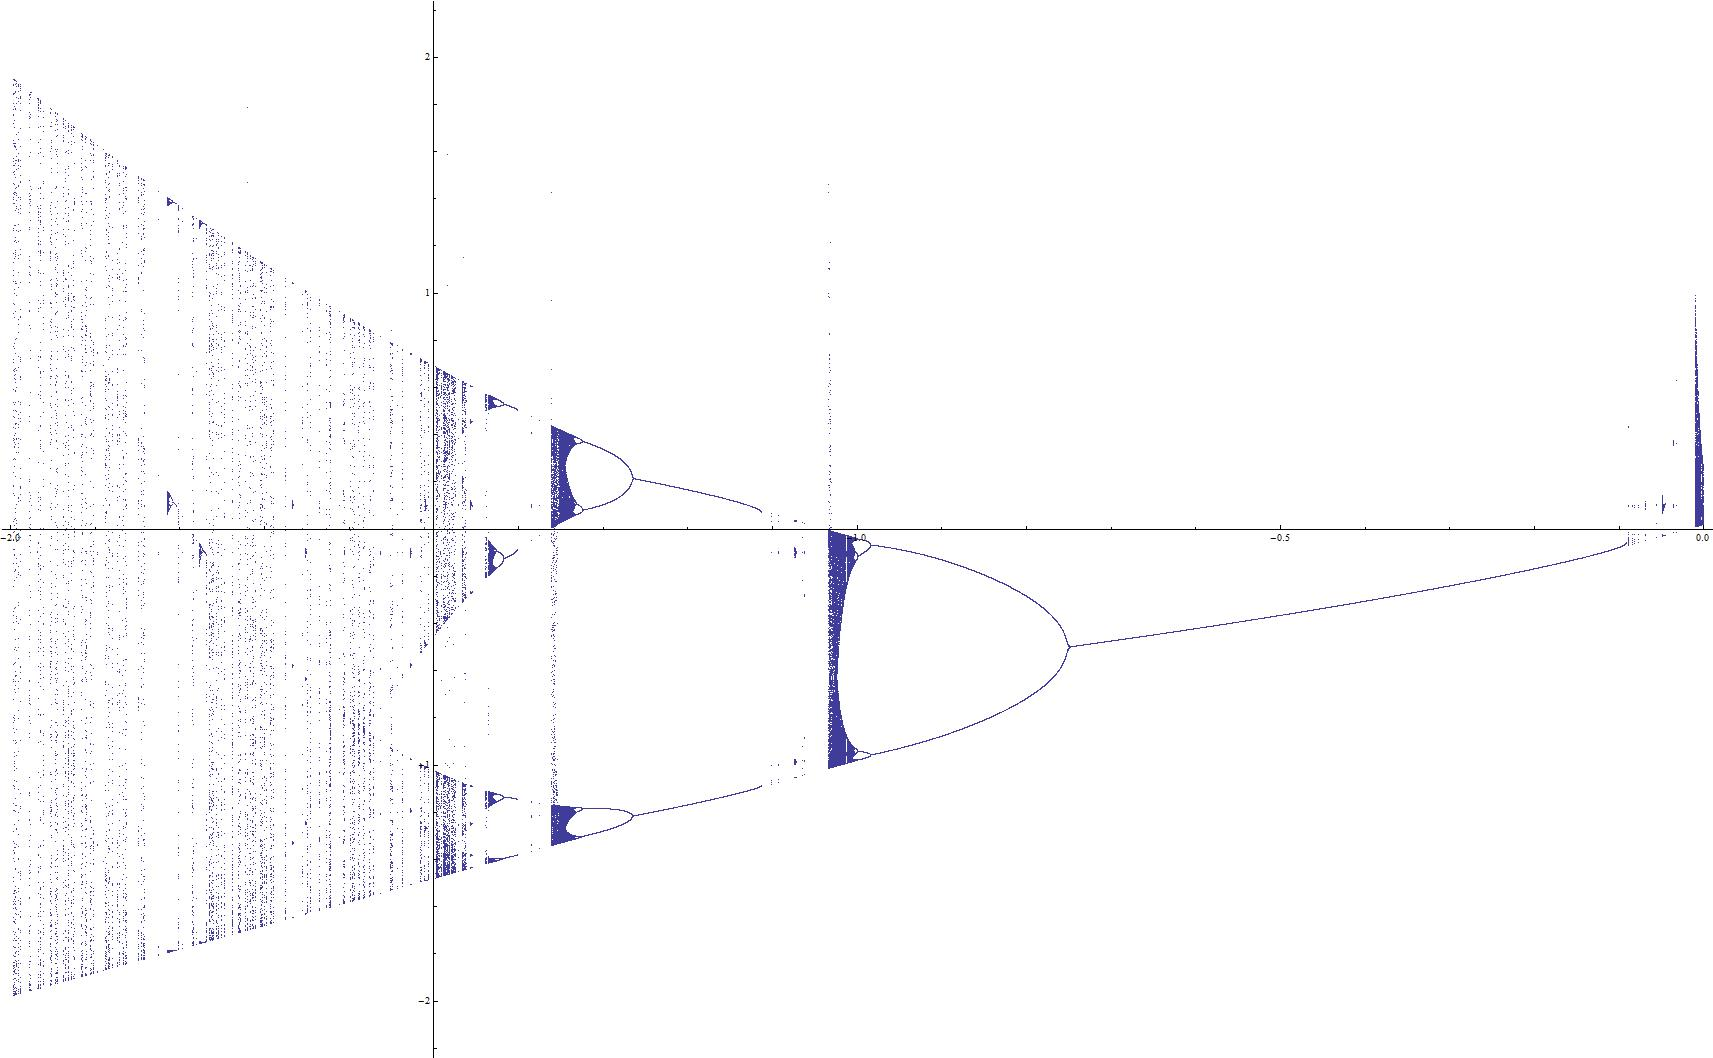
\includegraphics[width=.6\textwidth]{orbit_real_beta0001.jpg}\caption{Orbit Diagram for $z^{2} + c + \frac{0.0001}{ \overline{z}^{2}}$ where $z$ and $c$ are real}\end{figure}

\begin{figure}[H]\centering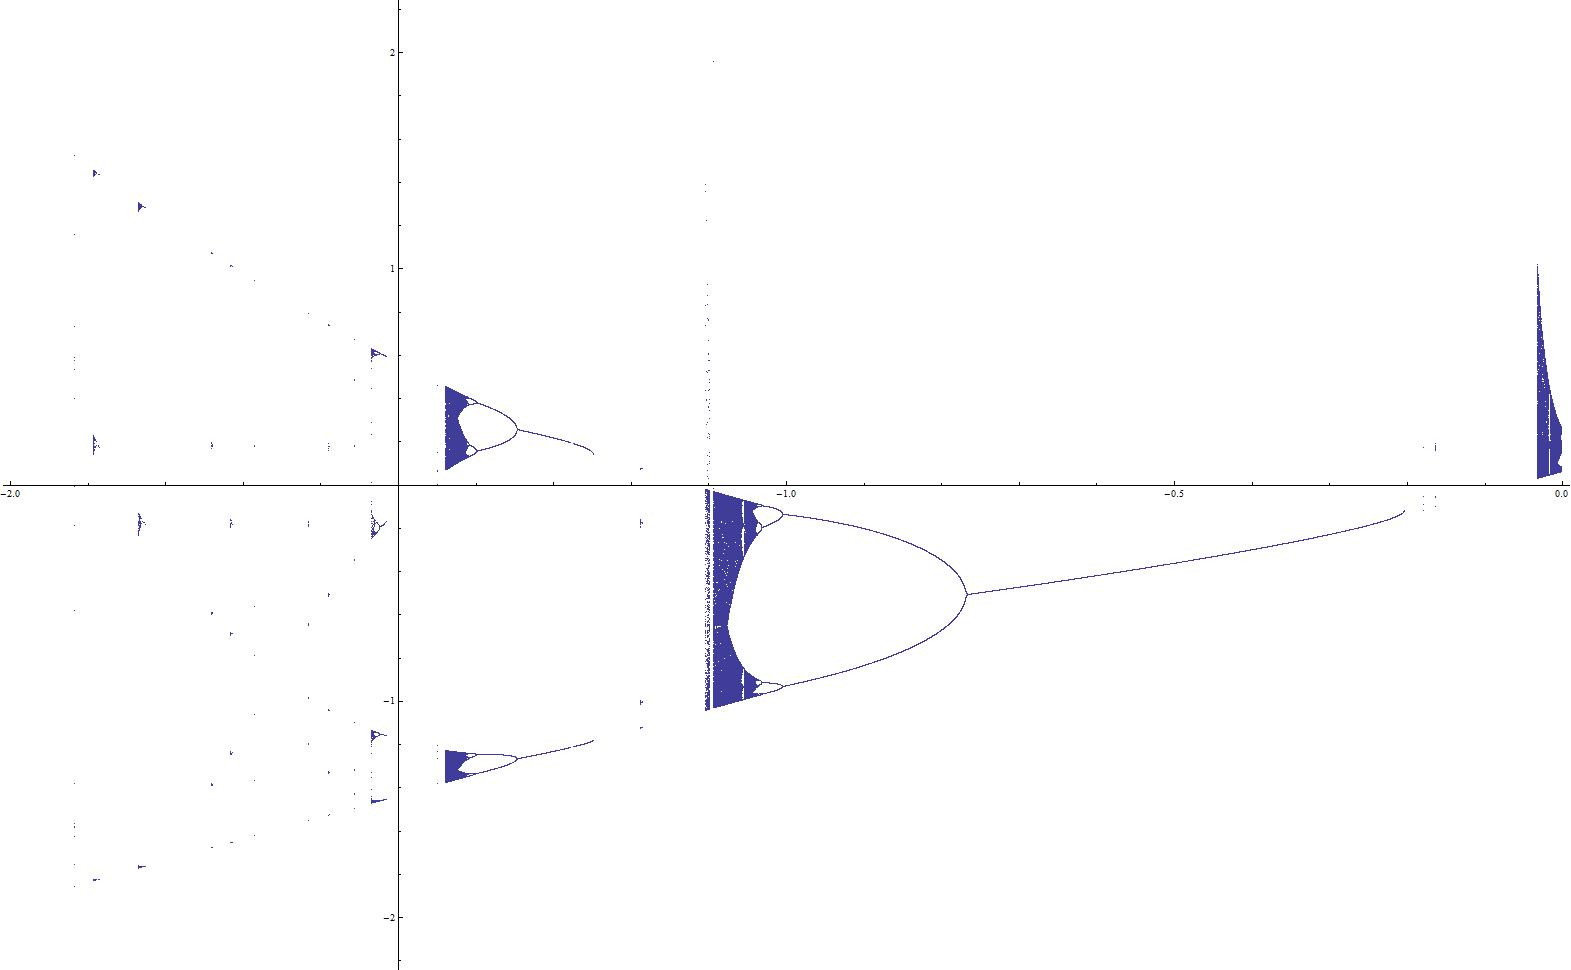
\includegraphics[width=.6\textwidth]{orbit_real_beta001.jpg}\caption{Orbit Diagram for $z^{2} + c + \frac{0.001}{ \overline{z}^{2}}$ where $z$ and $c$ are real}\end{figure}

\begin{figure}[H]\centering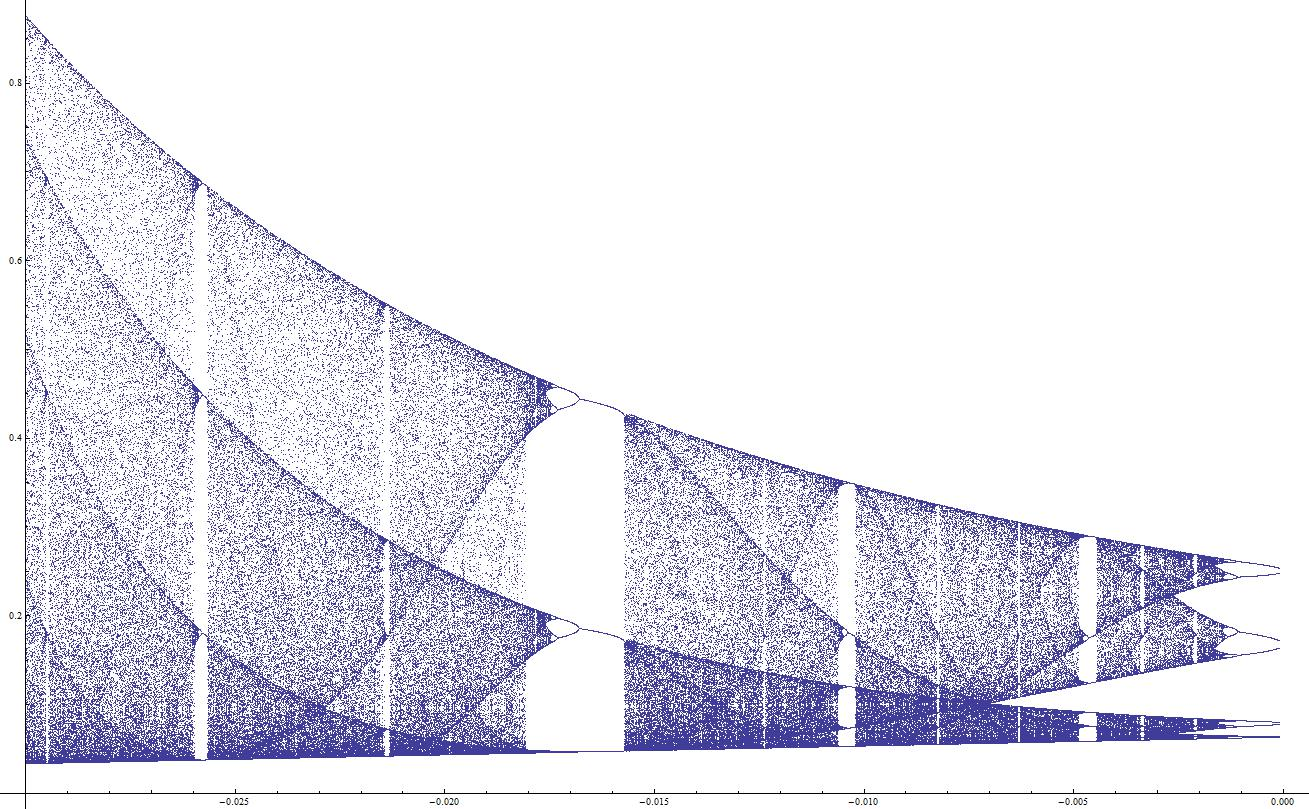
\includegraphics[width=.6\textwidth]{orbit_real_beta001_zoom.jpg}\caption{Zoom on orbit Diagram for $z^{2} + c + \frac{0.01}{ \overline{z}^{2}}$ where $z$ and $c$ are real}\end{figure}

\begin{figure}[H]\centering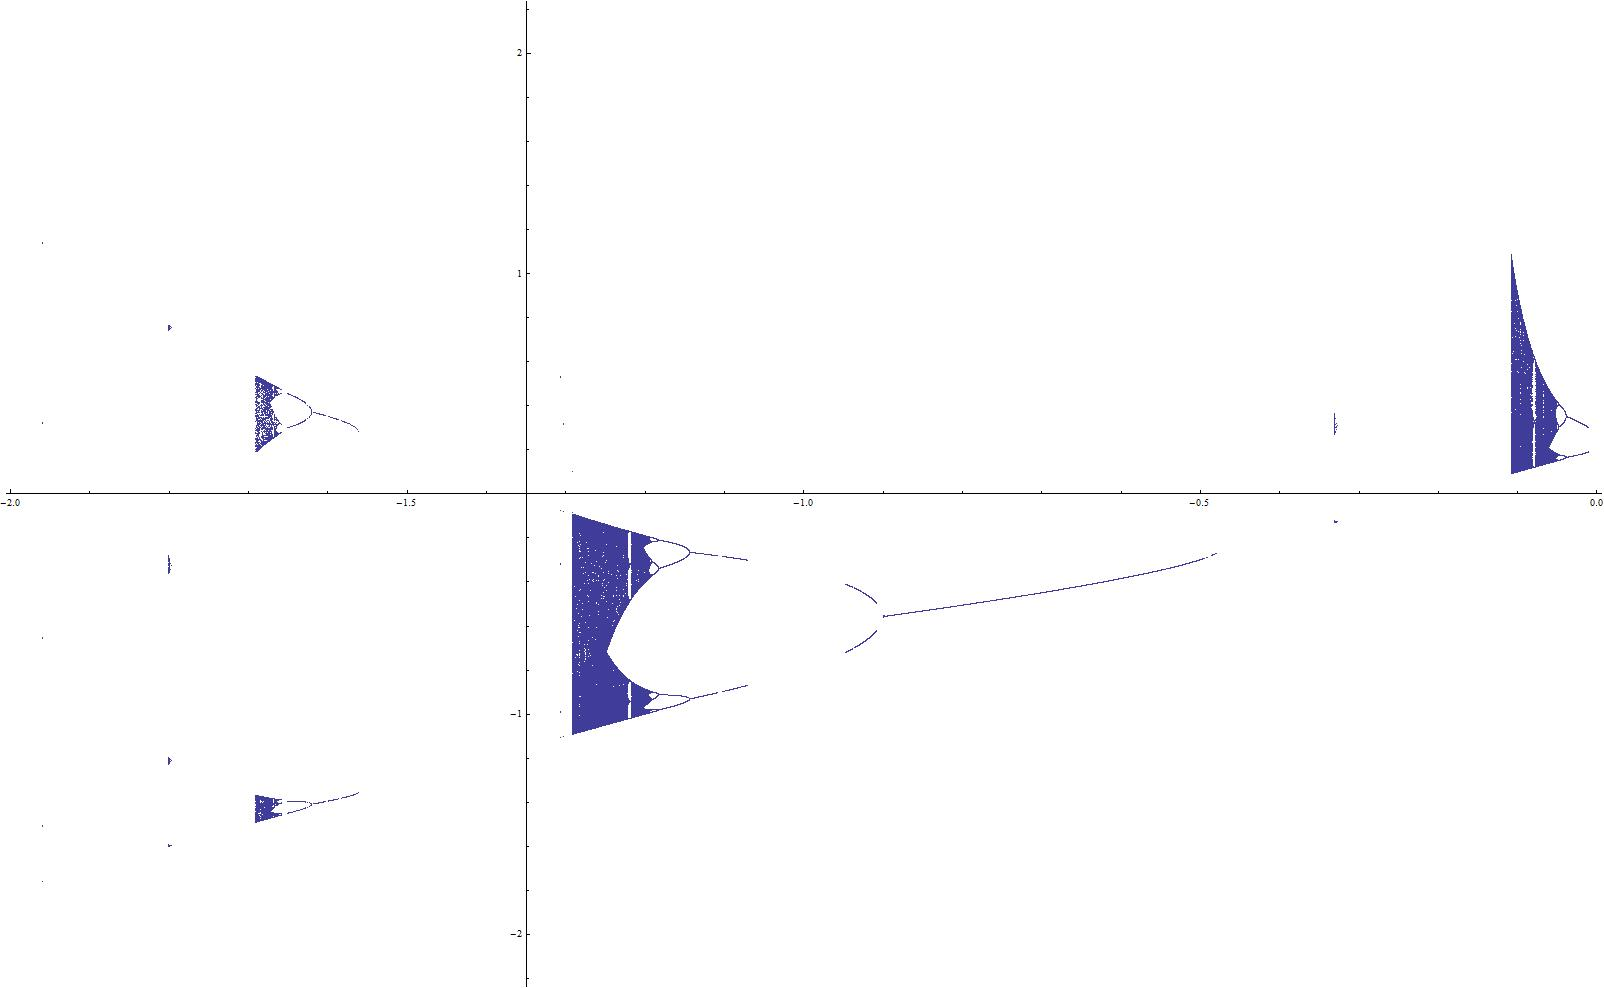
\includegraphics[width=.6\textwidth]{orbit_real_beta01.jpg}\caption{Orbit Diagram for $z^{2} + c + \frac{0.01}{ \overline{z}^{2}}$ where $z$ and $c$ are real}\end{figure}

\begin{figure}[H]\centering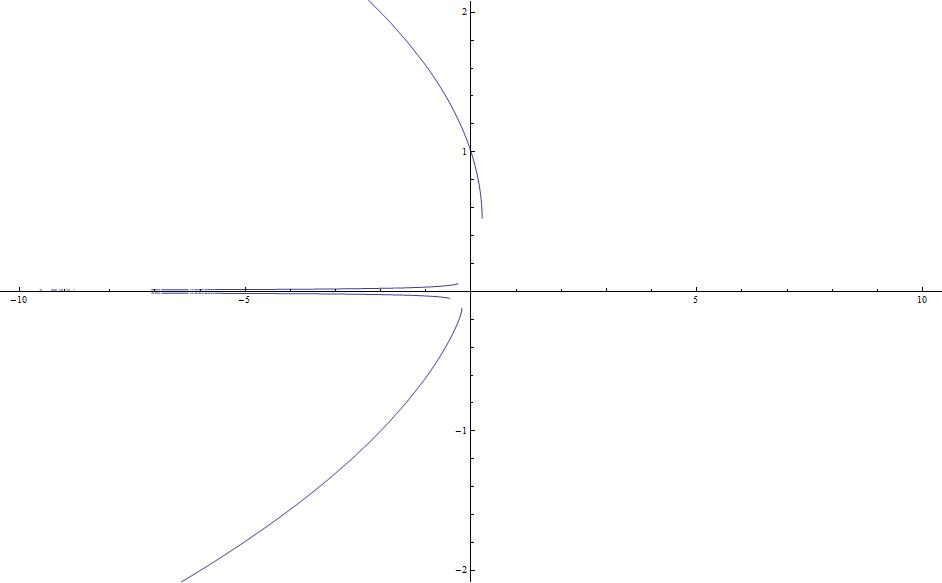
\includegraphics[width=.6\textwidth]{fixed_points_real_001.jpg}\caption{Fixed points for $z^{2} + c + \frac{0.001}{ \overline{z}^{2}}$ where $z$ and $c$ are real}\end{figure}

\begin{figure}[H]\centering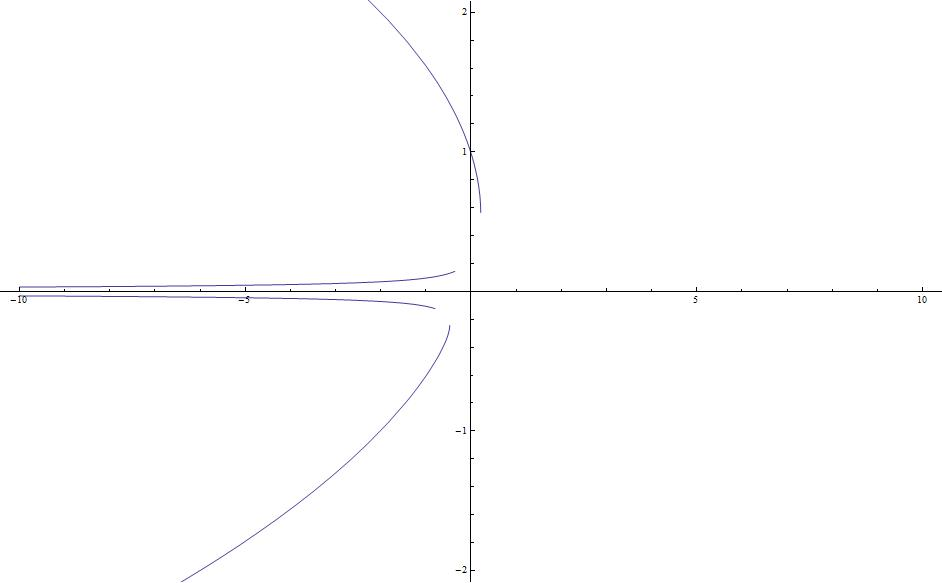
\includegraphics[width=.6\textwidth]{fixed_points_real_01.jpg}\caption{Fixed points for $z^{2} + c + \frac{0.01}{ \overline{z}^{2}}$ where $z$ and $c$ are real}\end{figure}

\begin{figure}[H]\centering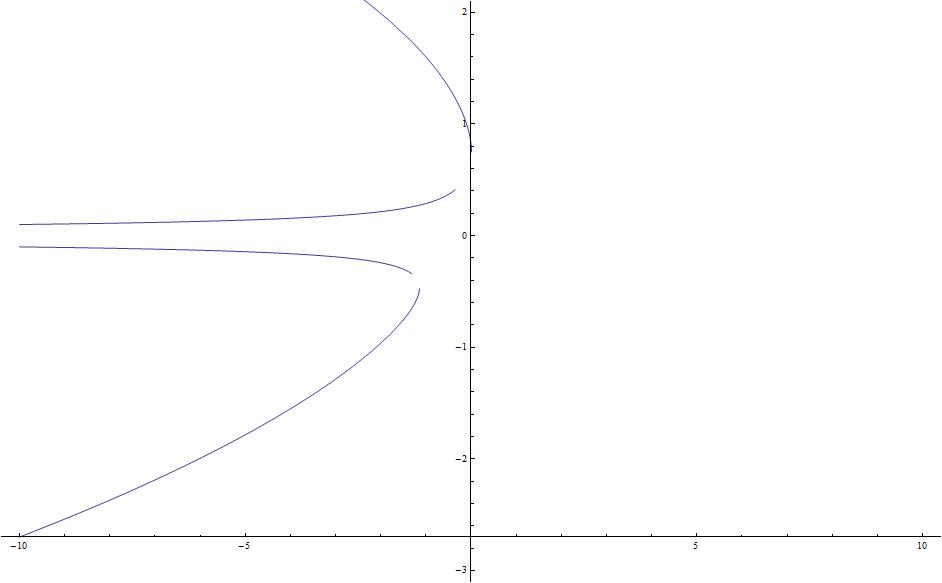
\includegraphics[width=.6\textwidth]{fixed_points_real_1.jpg}\caption{Fixed points for $z^{2} + c + \frac{0.1}{ \overline{z}^{2}}$ where $z$ and $c$ are real}\end{figure}

\begin{figure}[H]\centering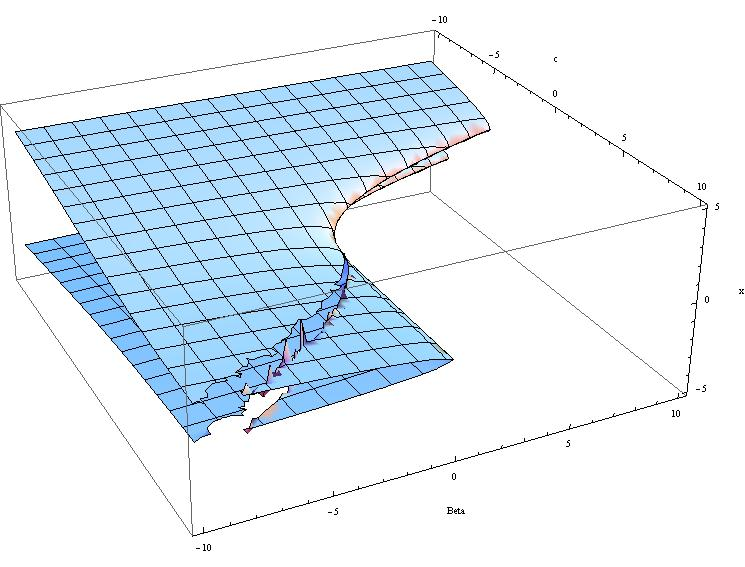
\includegraphics[width=.6\textwidth]{fixed_points_real_view1.jpg}\caption{A view of the fixed points for $z^{2} + c + \frac{\beta}{ \overline{z}^{2}}$ where $z$, $c$, and $\beta$ are real}\end{figure}

\begin{figure}[H]\centering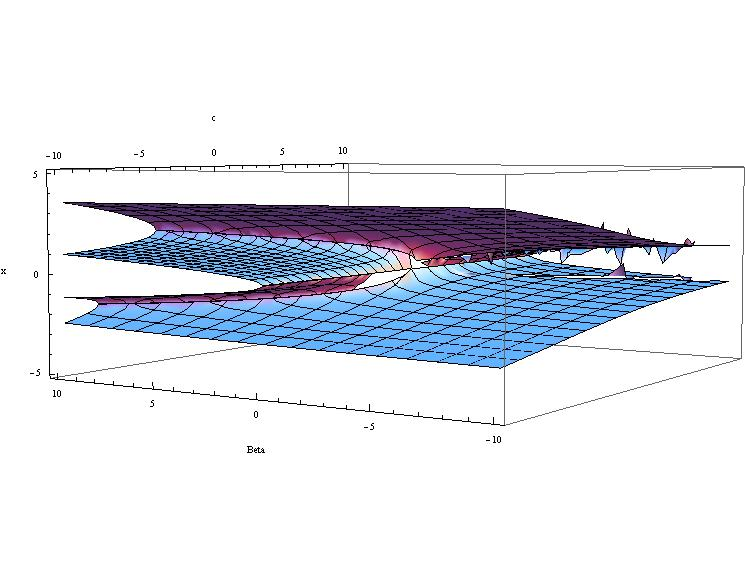
\includegraphics[width=.6\textwidth]{fixed_points_real_view2.jpg}\caption{A view of the fixed points for $z^{2} + c + \frac{\beta}{ \overline{z}^{2}}$ where $z$, $c$, and $\beta$ are real}\end{figure}





\section{Preliminary Write-Ups}
\subsection{}

\subsection{Real Splines}

As a way of restricting the scope of initial solution attempts, we will focus our attention on the dynamics of the real axis. Thus we have the following simplification:
\[
	x^d + c + \frac{\beta}{\overline{x}^n} \Rightarrow x^d + c + \frac{\beta}{x^n}
\]
Then if we make the simplifying assumption that $n = d$ and choose different $\beta$ values, we can start to solve for the fixed points of the system.

\underline{$d = 1$}



(AFTER ABOVE WORK) Thus we have begun to understand the dynamics of this system. However the above work only applies to the case where $x$ is real, $n = d$, and $n = d,$ and $\beta$ are specific values.
\end{document}